\documentclass[12pt, a4paper]{article}
    \usepackage[utf8]{inputenc}
    %\usepackage[english, spanish]{babel}
    %\usepackage{fullpage} % changes the margin
    \usepackage{graphicx} 
    \usepackage{enumitem} 
    \usepackage{chngcntr}
    \counterwithin{figure}{section}
    \renewcommand{\thesection}{\arabic{section}} 
    \renewcommand{\thesubsection}{\thesection.\arabic{subsection}}
    \renewcommand{\baselinestretch}{1.5}

    \usepackage{amsmath}
    \usepackage{mathptmx}
    \usepackage[spanish, es-tabla]{babel} %es-tabla añadido
    \usepackage{amssymb}
    \usepackage{makeidx}
    \usepackage{float}
    \pagenumbering{arabic}
    \usepackage[left=25mm, right=25mm, top=25mm, bottom=25mm]{geometry}

    \usepackage[backend=biber]{biblatex}
    \bibliography{referencias}

\begin{document}

    \begin{titlepage}
        \centering
        {\scshape\Large Universidad Central de Venezuela \par}
        {\scshape\Large Facultad de ingeniería \par}
        {\scshape\Large Escuela de ingeniería Eléctrica \par}
        {\scshape\Large Departamento de Electrónica, Computación y Control \par}

        \vspace{6cm}
        {\Large\bfseries Pre-Laboratorio 6 : Polarización del JFET\par}
        \vspace{6cm}

        \vfill
        \begin{flushright}
            Estudiante:\par
            Santana Ricardo C.I.:29571461 \par
            \vspace{1cm}  
        \end{flushright}
        \vfill
        {\large \today \par}
    \end{titlepage}

    \section{Introducción}

    Existen diversos tipos de transistores con distintas aplicaciones. Entre ellos, cabe destacar el transistor de efecto de campo (FET), el cual controla la corriente que circula por uno de sus pines a través del voltaje aplicado entre sus otros dos terminales.
    
    Comprender el funcionamiento de este dispositivo tanto estática como dinamicamente es de suma importancia, ya que su uso permite obtener ganancias de señal elevadas y una alta impedancia de entrada. Estas características resultan fundamentales en la amplificación de señales débiles y en la reducción de ruido en circuitos electrónicos. Los amplificadores JFET tienen variadas aplicaciones y se utilizan en diferentes áreas. Por ejemplo, son empleados en sistemas de audio de alta calidad, en instrumentos de medición y control de procesos industriales, así como en sistemas de comunicación inalámbrica, entre otros.

    En el siguiente prelaboratorio, se investigará el diseño y la implementación de un amplificador que utiliza un JFET, además se analizará los efectos sobre el punto de operación de la variación de su resistencia de drenaje mediante el uso de un potenciómetro.

    \newpage

    \section{Objetivos}

    \subsection{Objetivo General}
    \begin{itemize}
        \item Analizar el funcionamiento de un transistor JFET como amplificador.
    \end{itemize}

    \subsection{Objetivos Específicos}
    \begin{itemize}
        \item Estudiar el comportamiento dinámico de una estructura básica amplificadora JFET canal n.
        \item Obtener experimentalmente las características más importantes de un amplificador como son: la ganancia de tensión, impedancia de entrada e impedancia de salida.
    \end{itemize}

    \newpage

    \section{Marco Teórico}

    \subsection{Modelo de pequeña señal para transistores FET [1]}

    El circuito equivalente de pequeña señal de un transistor FET se puede obtener por métodos análogos a los utilizados en transistores bipolares. Sin embargo, al ser dispositivos controlados por tensión, el modelo bipuerta más adecuado es el de parámetros $\{Y\}$, ya que relacionan las corrientes de salida con tensiones de entrada. La figura \ref{fig:mt1} representa el modelo de pequeña señal de un FET constituido por dos parámetros: $g_m$, o factor de admitancia, y $r_d$, o resistencia de salida o resistencia de drenador. Esta notación es la más extendida para describir estos parámetros, aunque algunos fabricantes utilizan la notación en parámetros $\{Y\}$ o $\{G\}$, denominando $y_{fs}$ o $g_{fs}$ a $g_m$, e $y_{os}^{-1}$ o $g_{os}^{-1}$ o $r_oss$ a $r_d$. Estos parámetros dependen de la corriente de polarización del transistor (ID), y el fabricante proporciona las curvas que permiten extraer sus valores en diferentes condiciones de polarización. A continuación se describe con más detalle los parámetros $g_m$ y $r_d$.

    \begin{figure}[h!]
        \centering
        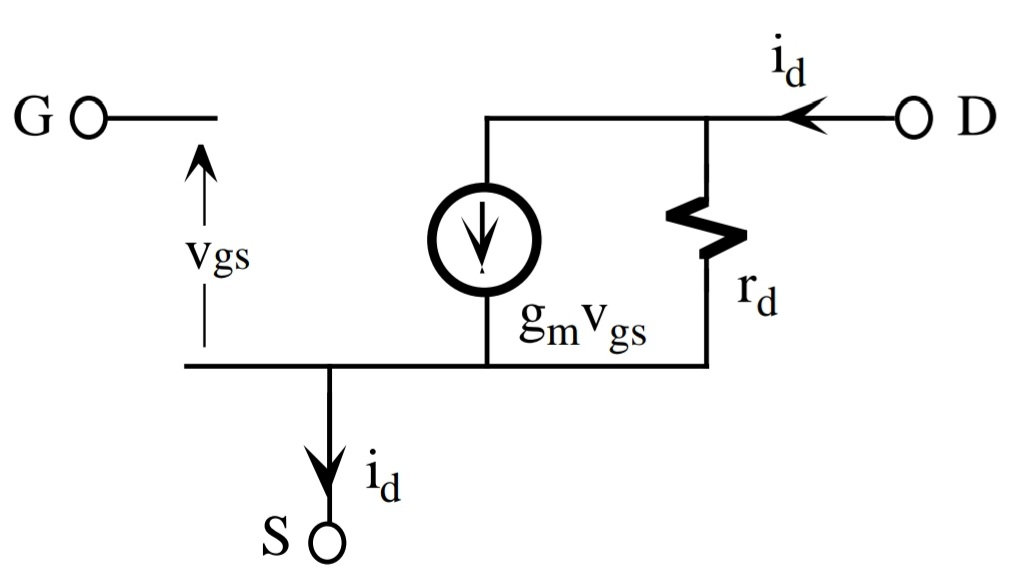
\includegraphics[height=5cm\textwidth]{pequenasenal.jpg}
        \caption{Modelo de pequeña señal de un transistor FET.}
        \label{fig:mt1}
    \end{figure}

    {\bf Factor de admitancia gm.} Se define este parámetro como

    \begin{equation} \label{eqgm}
        g_m = \left.\frac{\Delta I_D}{\Delta V_{GS}}\right|_{V_{DSQ}} = \left.\frac{I_{D2}-I_{D1}}{V_{GS2}-V_{GS1}}\right|_{V_{DSQ}} = \left.\frac{\Delta i_d}{\Delta v_{gs}}\right|_{V_{DSQ}}
    \end{equation}

    En un JFET, $g_m$ se puede extraer a partir de la ecuación analítica del transistor en la región de saturación que relaciona la $I_D$ con la $V_GS$, definida por

    \begin{equation} \label{eqvgs}
        I_D = I_{DSS}\left(1-\frac{V_{GS}}{V_P}\right)^2 \;\;\; ó \;\;\; 1-\frac{V_{GS}}{V_P} = \sqrt{\frac{I_D}{I_{DSS}}}
    \end{equation}

    En la ecuación \eqref{eqgm}, $g_m$ es un parámetro definido por cociente de incrementos que se pueden aproximar por derivadas, de forma que aplicando esta definición a la ecuación \eqref{eqvgs} y resolviendo se obtiene que

    \begin{equation} \label{eqdgm}
        g_m = \left.\frac{d I_D}{d V_{GS}}\right|_{V_{DSQ}} = -\frac{2I_{DSS}}{V_P}\left(1-\frac{V_{GS}}{V_P}\right) = -\frac{2}{V_P}\sqrt{I_DI_{DSS}}
    \end{equation}

    {\bf Resistencia de salida o de drenador rd.} Se define como

    \begin{equation} \label{eqrd}
        r_d = \left.\frac{\Delta V_{DS}}{\Delta I_D}\right|_{V_{GSQ}} = \left.\frac{V_{DS2}-V_{DS1}}{I_{D2}-I_{D1}}\right|_{V_{GSQ}} = \left.\frac{\Delta v_{ds}}{\Delta i_d}\right|_{V_{GSQ}}
    \end{equation}

    Factor de amplificación $\mu$. Relaciona los parámetros $g_m$ y $r_d$ de la siguiente manera

    \begin{equation} \label{eqmu}
        \mu = \frac{\Delta V_{DS}}{\Delta V_{GS}} = \frac{\Delta I_D}{\Delta V_{GS}}\frac{\Delta V_{DS}}{\Delta I_D} = g_mr_d
    \end{equation}

    Las definiciones gráficas de $g_m$ y $r_d$ se encuentran en las figuras \ref{fig:mt2} y \ref{fig:mt3}.

    \begin{figure}[h!]
        \centering
        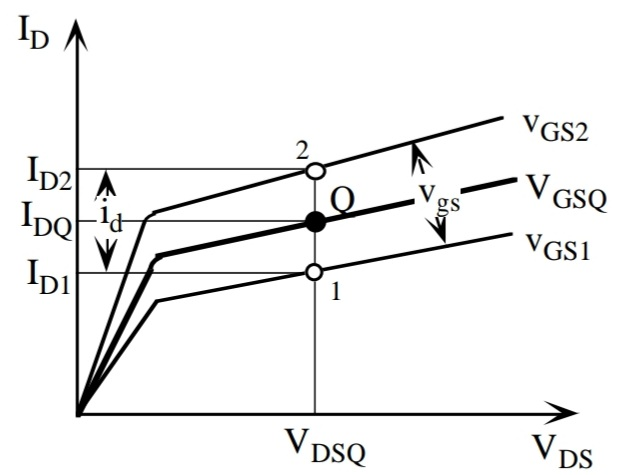
\includegraphics[height=5cm\textwidth]{grafgm.jpg}
        \caption{Definición gráfica de $g_m$.}
        \label{fig:mt2}
    \end{figure}

    \begin{figure}[h!]
        \centering
        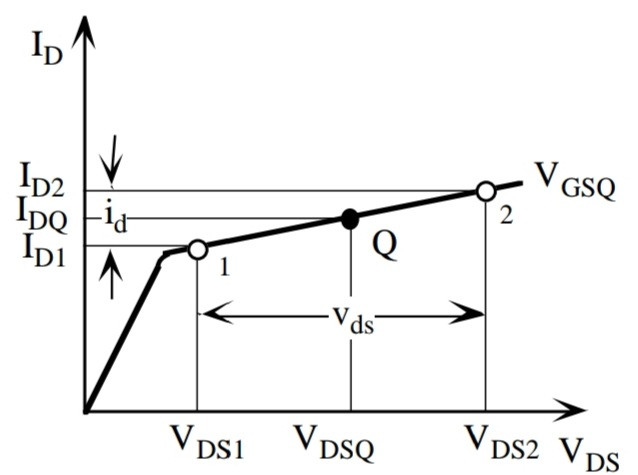
\includegraphics[height=5cm\textwidth]{grafrd.jpg}
        \caption{Definición gráfica de $r_d$.}
        \label{fig:mt3}
    \end{figure}

    En la \ref{tab:mt1} se resume los configuraciones más utilizadas de amplificadores básicos basados en transistores FET, bien sea JFET o MOSFET. Estas configuraciones son: fuente común, fuente común con resistencia de fuente, puerta-común y drenador común. Las ecuaciones indicadas en la derecha permite obtener el modelo equivalente en tensión de los diferentes circuitos. Un FET operando en fuente común presenta la mayor ganancia en tensión aunque ésta sea muy inferior a los valores de E-C en transistores bipolares. La configuración drenador común tiene una ganancia ligeramente inferior a 1, similar al C-C en transistores bipolares.

    \begin{table}[h!]
        \centering
        \caption{Análisis de las configuraciones básicas de los amplificadores JFET y MOSFET.} 
        \label{tab:mt1}
        \begin{tabular}{c}
            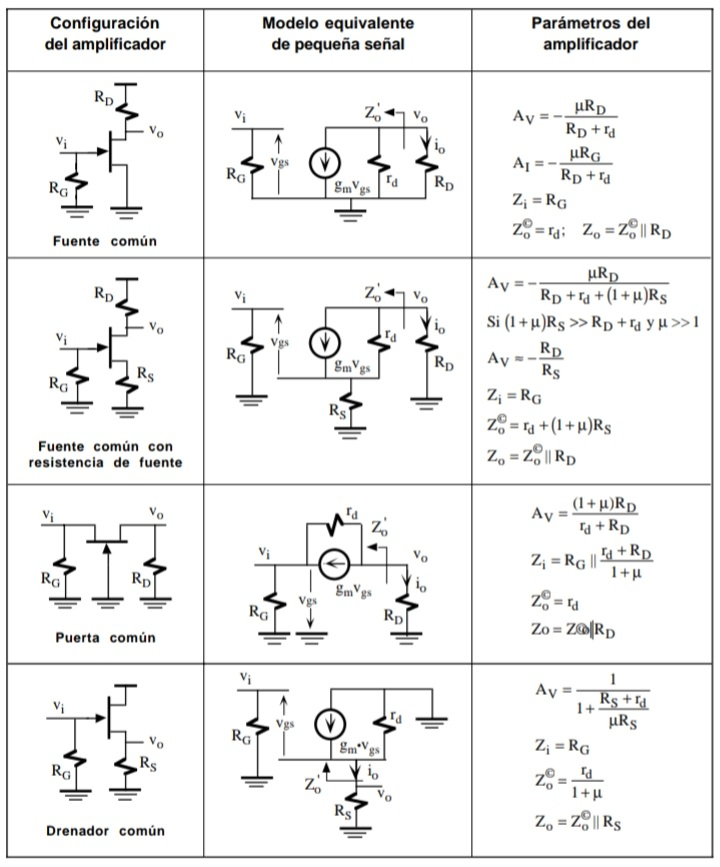
\includegraphics[width=16cm\textwidth]{configuraciones.jpg} \\
        \end{tabular}
    \end{table}

    \newpage

    \section{Metodología}

    \subsection{Trabajo Previo al Laboratorio}

    Para el circuito de la Figura \ref{fig:amp}:

    \begin{figure}[h!]
        \centering
        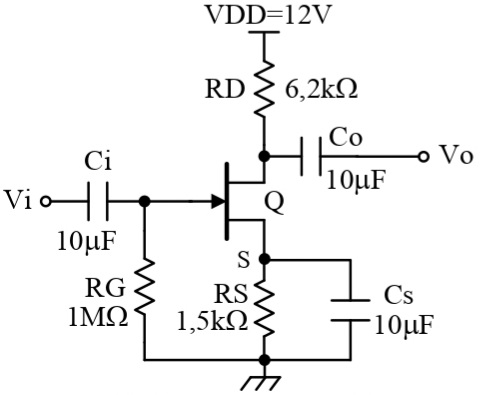
\includegraphics[height=5cm\textwidth]{amplificador.jpg}
        \caption{Amplificador JFET}
        \label{fig:amp}
    \end{figure}

    Calcular:

    \begin{enumerate}
        \item \label{p11}	Punto estático de operación(I_{DQ}, V_{DSQ}).
        \item \label{p12}	La ganancia de tensión Av, Impedancia de entrada Zin e Impedancia de salida Zout.
    \end{enumerate}

    \subsection{Trabajo de Laboratorio}

    \begin{enumerate}
        \item \label{p21}   Mida el punto estático de operación.
        \item \label{p22}	Coloque en el generador una señal senoidal de frecuencia 1kHz, promedio nulo y amplitud 1Vp-p.
        \item \label{p23} 	Observe, con el osciloscopio en doble canal, las formas de onda de la entrada Vi y la salida Vo. Dibuje ambas formas de onda para luego en el informe,en el punto del análisis de resultados, las compare en cuanto a su forma, frecuencia y amplitud. Mida la tensión de entrada y de salida pico-pico.
        \item \label{p24} 	Suba la amplitud de la señal de entrada hasta el punto donde comienza a distorsionarse la señal de salida. Mida la amplitud pico-pico de la señal de entrada. Dibuje ambas formas de onda.
        \item \label{p25} 	Suba hasta el máximo la amplitud de la señal de entrada y mida esta amplitud pico-pico. Dibuje las ondas de entrada y salida.
        \item \label{p26} Mida experimentalmente los valores de tensiones para luego de terminar en el informe las impedancias de entrada y desalida del amplificador.
    \end{enumerate}

    \newpage

    \section{Cálculos prévios}

    Se trabajará con el transistor FET canal n 2N5555, el cual posee las siguientes especificaciones:
    
    \begin{table}[h!]
        \centering
        \caption{Características del transistor 2N5555} %nombre de la tabla
        \label{tab:5555} %indice de la tabla
        \begin{tabular}{c}
            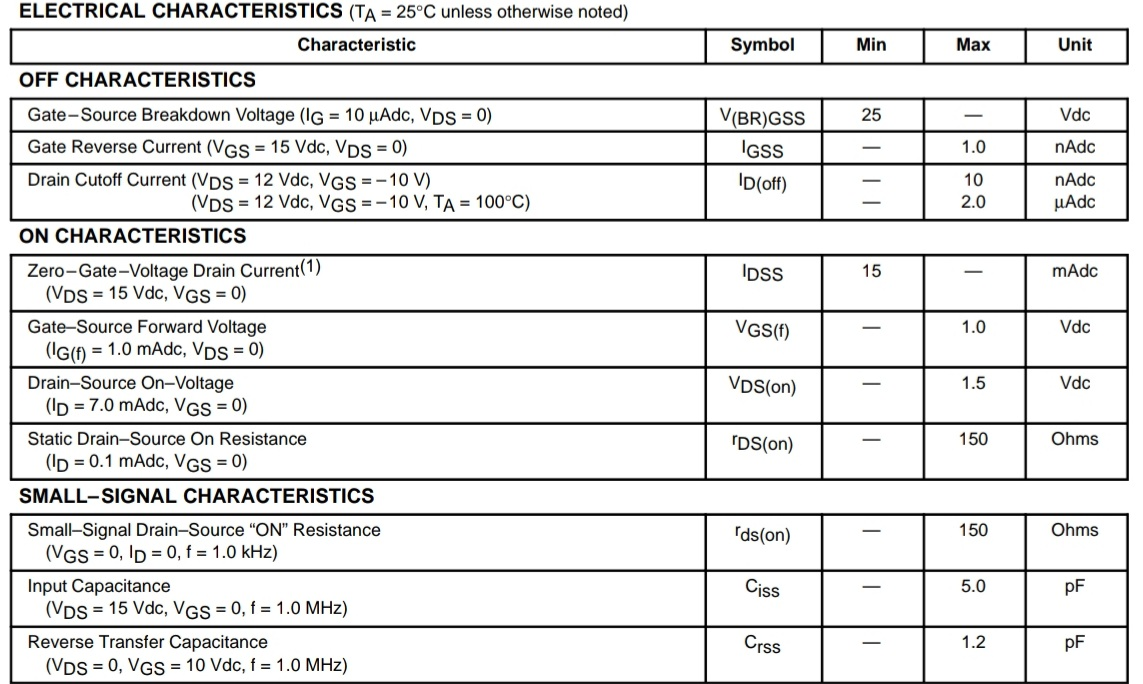
\includegraphics[width=16cm\textwidth]{2N5555.jpg} \\
        \end{tabular}
    \end{table}
    
    de las cuales se deduce por promediación que:

    $V_P = -1V$

    $I_{DSS} = 15mA$

    Entonces analizando el circuito de la figura \ref{fig:cir1}, para encontrar el punto estático de operación $Q(V_{DSQ},I_{DQ})$, donde los condensadores se desacoplan por estar trabajando en DC.

    \begin{figure}[h!]
        \centering
        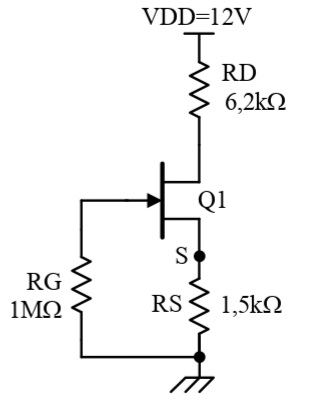
\includegraphics[height=5cm\textwidth]{circuito1.jpg} \par
        Figura \ref{fig:cir1}. Polarización del JFET canal n.
    \end{figure}

    Se tiene un JFET autopolarizado. Esto es debido a que la corriente circulando por $R_G$ es cero y, por tanto, toda la corriente ($I_D$) que entra por el drenador D sale por la fuente S.

    Analizando la malla relacionada al circuito de la compuerta con $I_G = 0$,

    $$V_{GS} = -I_DR_S \rightarrow I_D = -{V_{GS} \over R_S}$$

    \begin{equation} \label{eq1}
        I_D = -{V_{GS} \over R_S}
    \end{equation}

    Conociendo la características de transferencia de un JFET que relaciona $V_{GS}$ e $I_D$ por la fórmula \eqref{eqvgs}

    \begin{equation*}
        I_D = I_{DSS}\left( 1-{V_{GS} \over V_P}\right) ^2
    \end{equation*}

    Entonces

    $$I_{DQ} = I_{DSS}\left( 1-{V_{GSQ} \over V_P}\right) ^2 = -{V_{GSQ} \over R_S}$$

    buscando $V_{GSQ}$
    
    \begin{equation}
        \label{eq3}
        \begin{split}
            I_{DSS}\left( 1-{V_{GSQ} \over V_P}\right) ^2  & = -{V_{GSQ} \over R_S} \\
            1 - 2{V_{GSQ} \over V_P} + ({V_{GSQ} \over V_P})^2  & = -{V_{GSQ} \over I_{DSS}R_S} \\
            1 - 2{V_{GSQ} \over V_P} + {V_{GSQ}^2 \over V_P^2} + {V_{GSQ} \over I_{DSS}R_S} & = 0 \\
            {1 \over V_P^2}V_{GSQ}^2 + \left({1 \over I_{DSS}R_S} - {2 \over V_P}\right)V_{GSQ} + 1 & = 0 \\
        \end{split}
    \end{equation}

    Reemplazando valores conocidos en \eqref{eq3} y resolviendo ecuación de segundo grado

    \begin{split}
        {1 \over V_P^2}V_{GSQ}^2 + \left({1 \over I_{DSS}R_S} - {2 \over V_P}\right)V_{GSQ} + 1 & = 0 \\
        {1 \over (-1V)^2}V_{GSQ}^2 + \left({1 \over (15mA)(1.5k\Omega)} - {2 \over (-1V)}\right)V_{GSQ} + 1 & = 0 \\
        V_{GSQ}^2 + {92 \over 45}V_{GSQ} + 1 & = 0 \\
    \end{split}

    $$V_{GSQ} = -0.81V$$

    %\begin{figure}[h!]
    %    \centering
    %    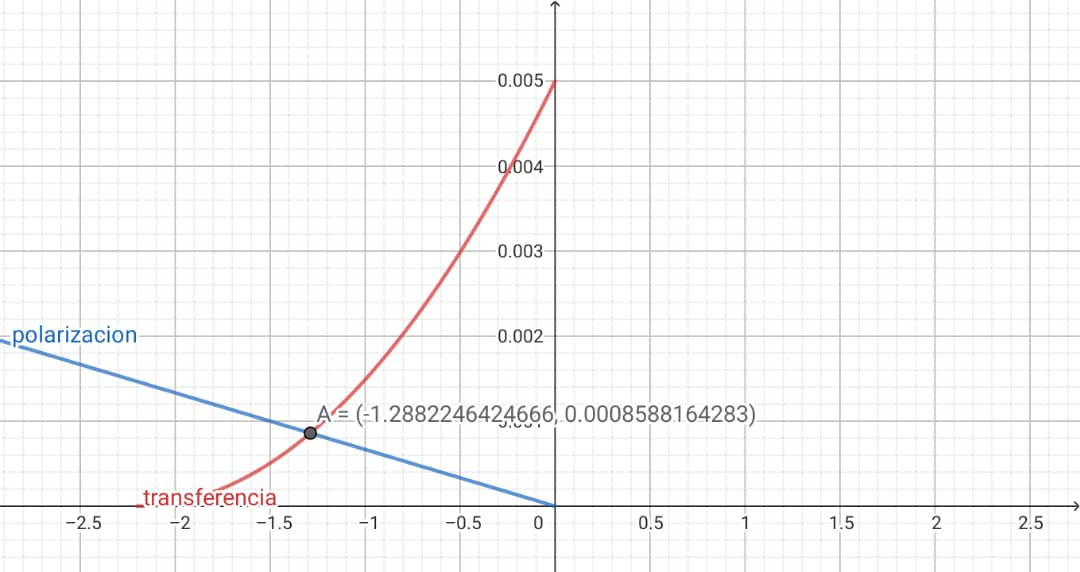
\includegraphics[height=5cm\textwidth]{graficoQ.jpg}
    %    \caption{Intersección de las ecuaciones \eqref{eq1} y \eqref{eq2}}
    %    \label{fig:vgsq}
    %\end{figure}

    Sustiyendo en \eqref{eq1}

    $$I_{DQ} = -{V_{GSQ} \over R_S} = -{(-0.8V) \over 1.5k\Omega} = 0.533mA$$

    Analizando malla relacionada al drenador

    $$V_{DD} = I_DR_D + V_{DS} + I_DR_S$$

    Particularizando para calcular $V_{DSQ}$

    \begin{equation}
        \label{eq4}
        \begin{split}
            V_{DD} & = I_{DQ}R_D + V_{DSQ} + I_{DQ}R_S \\
            I_{DQ}R_D + V_{DSQ} + I_{DQ}R_S & = V_{DD} \\
            V_{DSQ} & = V_{DD} - I_{DQ}(R_D + R_S)
        \end{split}
    \end{equation}
    
    Reemplazando valores en \eqref{eq4}

    $$V_{DSQ} = 12V - 0.533mA(6.2 + 1.5)k\Omega = 7.89V$$

    Punto de operacion

    $$Q : (7.89V, 0.533mA)$$

    Entonces el transistor se encuentra en zona de saturación
    
    Para el cálculo de la ganancia de tensión Av, Impedancia de entrada Zin e Impedancia de salida Zout se implementará el modelo del JFET para para pequeña señal que se observa en la figura \ref{fig:mt1}, donde los condensadores a media-alta frecuencia pasan a ser un corto, además para una aproximación se asumirá $r_d$ muy alta, es decir, un abierto.

    Quedando como modelo dinámico la Figura \ref{fig:din}

    \begin{figure}[h!]
        \centering
        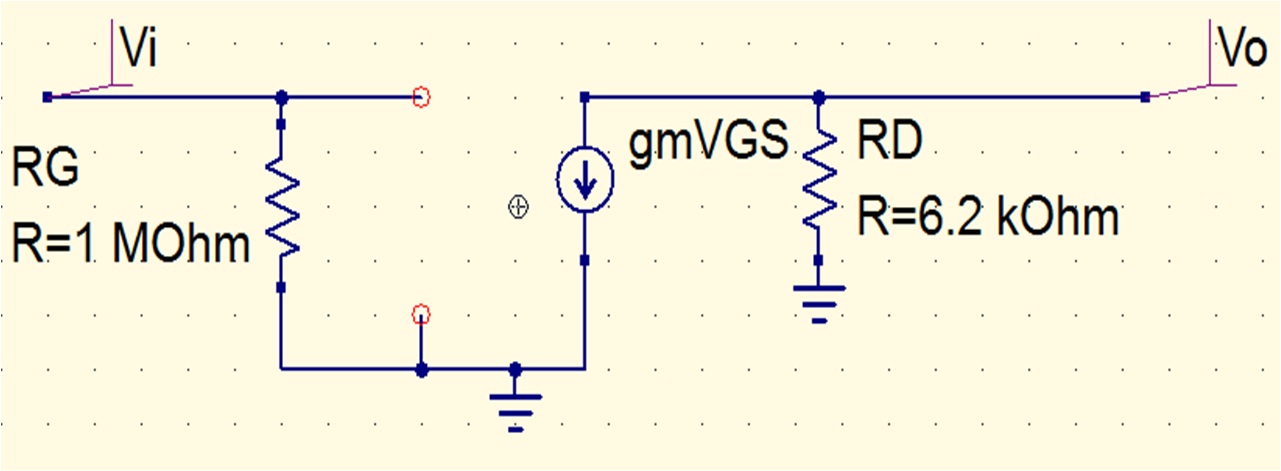
\includegraphics[width=15cm\textwidth]{dinamico.png}
        \caption{Modelo de circuito amplificador \ref{fig:amp} para pequeña señal con JFET}
        \label{fig:din}
    \end{figure}

    Sabiendo que la ganancia de tensión es

    \begin{equation} \label{eqgan}
        A_V = \frac{V_o}{V_i}
    \end{equation}

    donde

    \begin{equation*}
        \begin{split}
            V_o & = -g_mV_{GS}R_D \\
            V_i & = V_{GS}
        \end{split}
    \end{equation*}

    Sustituyendo en \eqref{eqgan} se tiene

    \begin{equation} \label{eqganp}
        A_V = \frac{-g_mV_{GS}R_D}{V_{GS}} = -g_mR_D
    \end{equation}

    Implementando la ecuación \eqref{eqdgm} deducida en el marco teórico

    $$g_m = -\frac{2}{V_P}\sqrt{I_DI_{DSS}}$$

    Al trabajar alrededor del punto estático de operacion

    $$g_m = -\frac{2}{-1V}\sqrt{(0.533mA)(15mA)} = 5.655 m\mho$$

    Quedando así la ganancia en \eqref{eqganp}

    $$A_V = -g_mR_D = -(5.655 m\mho)(6.2 k\Omega) = 35 V/V$$

    De la figura \ref{fig:din} se establece que

    \begin{equation*}
        \begin{split}
            A_V & = 35 V/V \\
            Z_i & = R_G = 1M\Omega \\
            Z_i & = R_D = 6.2k\Omega
        \end{split}
    \end{equation*}

    \newpage

    \section{Materiales e Instrumentos}

    %hay que realizar tablas

    \begin{itemize}
        \item Transistor FET canal n 2N5555
        \item Resistencia de carbon de $6.2k\Omega$  serie del $5\%$ y potencia de $1/4$ W.
        \item Resistencia de carbon de $1.5k\Omega$  serie del $5\%$ y potencia de $1/4$ W.
        \item Resistencia de carbon de $1M\Omega$  serie del $5\%$ y potencia de $1/4$ W.
        \item Capacitores electrolíticos de $10\mu F$ y $25V$
    \end{itemize}

\end{document}